% Sandia National Laboratories is a multimission laboratory managed and
% operated by National Technology & Engineering Solutions of Sandia, LLC, a
% wholly owned subsidiary of Honeywell International Inc., for the U.S.
% Department of Energy’s National Nuclear Security Administration under
% contract DE-NA0003525.

% Copyright 2002-2020 National Technology & Engineering Solutions of Sandia,
% LLC (NTESS).

 
The simulation of control systems, such as those used in power grids,
may require two different types of limiters for ``hard limits''.  They
are known as ``windup'' and ``anti-windup'' limiters ~\cite{Milano},
and are typically depicted as shown in Figures \ref{figAntiWindupLimiter} 
and \ref{figWindupLimiter}. The anti-windup limiter has the following 
equations:
\[
  \begin{array}{ll} 
  \mbox{if} \; x \geq x^{max} \; \mbox{and} \; \dot{x} \geq 0 \Rightarrow x = x^{max} \; \mbox{and} \; \dot{x} = 0\\
  \mbox{if} \; x \leq x^{min} \; \mbox{and} \; \dot{x} \leq 0 \Rightarrow x = x^{min} \; \mbox{and} \; \dot{x} = 0\\
  \mbox{otherwise} \; x = (y-x)/T
  \end{array}
\]
The anti-windup limiter has simultaneous constraints on both the output-voltage
level and the first derivative of the output-voltage level.  These equations were 
approximated with a \Xyce{} device model, as described below.  

\begin{figure}[ht]
  \centering
  \scalebox{1.0}
  {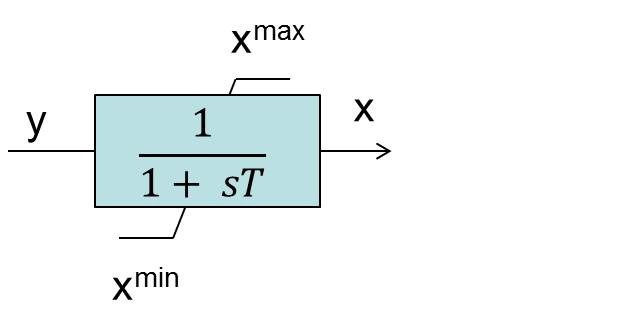
\includegraphics[width=2.1in,height= 1.05in]{AntiWindupLimiter.jpg}}
  \caption[Anti-Windup Limiter]{Anti-Windup Limiter. \label{figAntiWindupLimiter}}
\end{figure}

The windup limiter only has a constraint on the output-voltage level.  This is 
straightforward to implement with existing \Xyce{} device models.  The equations
and an example implementation are given below after the description of the \Xyce{} 
anti-windup limiter device model.

\begin{figure}[ht]
  \centering
  \scalebox{1.0}
  {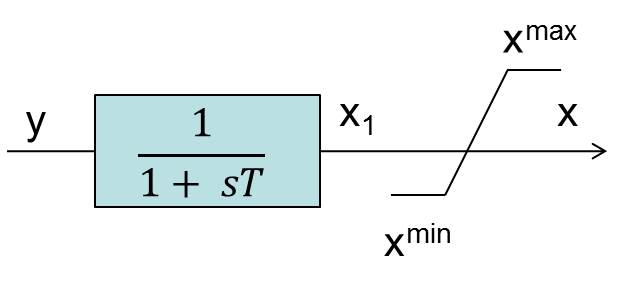
\includegraphics[width=2.0in,height= 1.0in]{WindupLimiter.jpg}}
  \caption[Windup Limiter]{Windup Limiter. \label{figWindupLimiter}}
\end{figure}

\begin{Device}\label{AntiWindupLimiter}

\device
\begin{alltt}
Y<type> <name> <input node> <output node> [device parameters] 
\end{alltt}
  
\examples
\begin{alltt}
YAntiWindupLimiter awl1 in1 out1 T=1 UL=0.5 LL=-0.5
YAWL awl2 in2 out2 T=2 UL=0.5 LL=-0.5
\end{alltt}

\parameters 
\begin{Parameters}
\param{type}
The device type has a verbose (\texttt{AntiWindupLimiter}) and a shortened
(\texttt{AWL}) form.  Their usage may be mixed within a netlist.

\param{name}
Name of the device instance.  This must be present, and unique amongst the 
\texttt{AntiWindupLimiter} devices in the netlist.

\param{input node}
There is one input node, \texttt{<input node>}. 

\param{output node}
There is one output node, \texttt{<output node>}.

\param{T} 
The time-constant, in seconds. 

\param{UL}
The upper control limit, in per-unit. The upper control limit must be 
greater than the lower control limit.  For numerical stability reasons,
the output signal level may exceed this upper limit slightly, depending 
on the time-steps used by \Xyce{}. The reason is that the derivative of 
the AWL output must be continuous in the current implementation of this 
device model.

\param{LL}
The lower control limit, in per-unit. For numerical stability reasons,
the output signal level may be slightly less than this lower limit, depending 
on the time-steps used by \Xyce{}. The reason is that the derivative of 
the AWL output must be continuous in the current implementation of this 
device model.
\end{Parameters}
\end{Device}

\paragraph{Anti-Windup Limiter Device Parameters}
%%
%% AntiWindupLimiter Table
%%
% This table was generated by Xyce:
%   Xyce -doc AntiWindupLimiter 1
%
\index{antiwinduplimiter!device instance parameters}
\begin{DeviceParamTableGenerated}{AntiWindupLimiter Device Instance Parameters}{AntiWindupLimiter_1_Device_Instance_Params}
LL & Lower Limit & per unit & -1 \\ \hline
T & Time Constant & s & 1 \\ \hline
UL & Upper Limit & per unit & 1 \\ \hline
\end{DeviceParamTableGenerated}



\paragraph{Branch Current and Power Accessors}
This version of the Anti-Windup Limiter device does not 
support the branch current accessor, \texttt{I()}, 
or the power accessors, \texttt{P()} or \texttt{W()}.

\paragraph{Comments}
The model parameters \texttt{UL} and \texttt{LL} are specified 
in ``per-unit'' since the AWL device was developed
for use with the power grid devices.  For other uses, the upper
and lower control limits can be considered to be specified in 
volts.

\paragraph{Windup Limiter}
For a first-order low-pass filter, followed by a hard-limiting function,
the windup limiter has the following equations and can be depicted
as shown in Figure \ref{figWindupLimiter}:
\[
x = \left\{ \begin{array}{ll}
x^{max}, &  \mbox{if} \; x_{1} \geq x^{max}\\
x, &  \mbox{if} \; x^{min} < x_{1} < x^{max}\\
x^{min}, & \mbox{if} \; x_{1} \leq x^{min}
\end{array}
\right.
\]
The version of the windup limiter shown in Figure \ref{figWindupLimiter}
can be implemented as a first-order RC filter followed by a B-Source with
a \texttt{LIMIT} function.  An example \Xyce{} netlist fragment is as follows:
\begin{alltt}
.param timeConstant=1
.param upperLimit=0.5
.param lowerLimit=-0.5
Rlpf y x1 {timeConstant}
Clpf x1 0 1
BLim x 0 V={LIMIT(V(x1),lowerLimit,upperLimit)}
\end{alltt}
